\documentclass[12pt]{article}
\usepackage{amssymb}
\usepackage[UTF8]{ctex}
\usepackage{geometry}
\usepackage{units}
\usepackage{pifont}
\geometry{
	a4paper,
	total={150mm,237mm},
	left=30mm,
	top=27mm,
	}
\usepackage{amsmath}
\usepackage{enumerate}
\usepackage{lipsum}
\usepackage{graphicx}
\usepackage{hyperref}
\usepackage{indentfirst}
\usepackage[graphicx]{realboxes}
\usepackage{booktabs}
\usepackage{cases}
\usepackage{subfig}  
\usepackage{float}
\usepackage{pythonhighlight}

\setlength{\parindent}{2em}
\title{HW11}
\author{姓名:陈锐林,学号:21307130148}

\begin{document}
\maketitle
\begin{large}
    \noindent Chapter37-HDD\\
\end{large}
Question1:\par
(1)以最复杂的7,30,8为例:首先需要转15°开始传输7,共用时15+30;之后寻道进入最内圈,花了40*2=80,需再转300-80=220,之后传输30,共花330;之后要再寻道出来,花80,这时和传输'8'的起始位置差50°,所以得转310,共花420。
所以在这三个阶段各花45,330,420。(2)而10,11,12,13就是分成两批次,不寻道+转+连续传输和寻道+转+传输。对于题目中的所有情况,结果如下:
\begin{tabular}{p{4cm}p{2cm}p{8cm}}  % 其中,tabular是表格内容的环境;c表示centering,即文本格式居中;c的个数代表列的个数
    \toprule[2pt]
    命令 & 用时 & 过程 \\ %中间用 & 隔开, 换行用\\
    \midrule[2pt]
    -a 0    & 195      & 0+165+30     \\
    -a 6    & 375 & 0+345+30 \\
    -a 30   & 375 & 80+265+30 \\
    -a 7,30,8     & 795 & (0+15+30)+(80+220+30)+(80+310+30) \\
    -a 10,11,12,13  & 585  & (0+105+30+30)+(40+320+30+30)\\
    \bottomrule[2pt]
\end{tabular}\\

\noindent Question4:\par
(1)FIFO中,很明显,像Question1讨论的,需要两次寻道,可能是增加了开销的。\par
(2)如果采用SSTF,过程应该如下:转15,连续传输"7","8",用时60,总共75;再寻道进入内圈,用时80,旋转190,传输30,用时300。总用时为375。
所以总结如下:对"7"为0+15+30;对"8"为0+0+30;对"30"为80+190+30。\\

\noindent Question10:\par
如果采用序列-a 20,11,25,那么这4种策略都会给出585的结果,因为他们总是把25放在最后解决。但如果用20-25-11的顺序就能用时更短。
具体过程如下:"20":40+5+30;"25":40+80+30;"11":80+190+30。共用时525。这说明贪心的策略并不总是最优的。
\newpage
\begin{large}
    \noindent Chapter38-RAID\\
\end{large}
Question1:\par
    (1)/(3)我使用了类似"python3 ./raid.py -n 5 -L 0 -R 20 -c -s 0"的指令来理解;其中-L取0,1,4,5,表示RAID level;-s取不同值表示不同随机种子。\par
    (2)对于RAID-5的左对称和左不对称问题,我使用这两条指令"python3 ./raid.py -n 5 -L 5 -R 20 -c -5 LS"和"python3 ./raid.py -n 5 -L 5 -R 20 -c -5 LA",
这个命令分别要求访问地址8,9,10,15,16。最后输出的结果和我认知的左对称和左不对称格局(如下)是一样的:排列时,左对称每行起始地址在上一行的检验和下,之后再补全;左不对称则直接
按从左到右的顺序排。
\begin{figure}[!h]
    \centering
    \subfloat[左对称]{\includegraphics[width=6.5cm,height=7.5cm]{P1.jpg} \label{X}}
    \hfill
    \subfloat[左不对称]{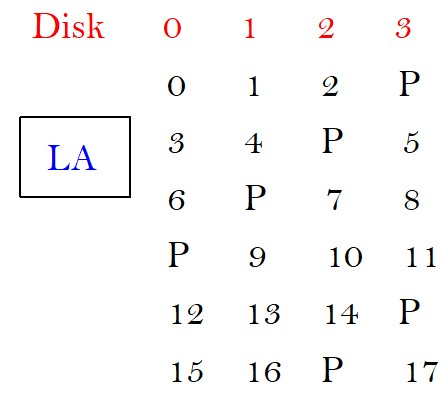
\includegraphics[width=6.5cm,height=7.5cm]{P2.jpg} \label{Y}}
\end{figure}\\
Question4:\par
(1)随着申请块的大小的增加,在读取时就要跨越Disks。对于RAID-0,如读地址8,就要用到D0(off-2),D1(off-2)。
对于RAID-1,可能就是读D0(off-4),D2(off-4)。RAID-4读取为D2(off-2),D0(off-0)。而对于RAID-5,如上面给出的,
左对称时就是D0(off-2),D1(off-3);左不对称时是D3(off-2),D1(off-3).
\begin{figure}[!h]
    \centering
    \subfloat[RAID-0]{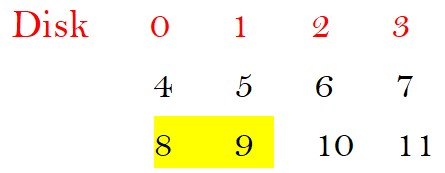
\includegraphics[width=4.5cm,height=3cm]{P3.jpg} \label{X}}
    \hfill
    \subfloat[RAID-1]{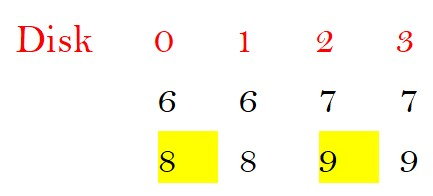
\includegraphics[width=4.5cm,height=3cm]{P4.jpg} \label{Y}}
    \hfill
    \subfloat[RAID-4]{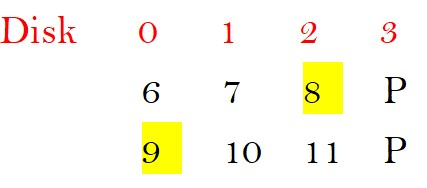
\includegraphics[width=4.5cm,height=3cm]{P5.jpg} \label{Z}}
\end{figure}\par
\newpage
(2)对于顺序读取的情况,设置大小为8K,就会读0,2,4,6,8,...;设置大小为12K,就会读取0,3,6,9,12,...;为了让I/O更加高效,在每一次的申请读数据时要让大小更大些,
比如这里可以采用12K和16K;让更多的磁盘同时动起来。


\end{document}